%% §1 — H-Matrix BEM Solver  (5 slides)
\section{H-Matrix BEM Solver}

%% ── Slide 1: The N² wall ────────────────────────────────────────────────────
\begin{frame}{The $N^2$ Wall}
\begin{columns}[T]
\begin{column}{0.48\textwidth}
  Surface contact requires \textbf{dense matrix–vector products}
  \[
    u_i = \sum_{j=1}^{N} S_{ij}\,p_j,
    \qquad S_{ij} = \frac{1}{\pi\Esta}
      \calL\!\left(\mathbf{x}_i{-}\mathbf{x}_j,\tfrac{h}{2}\right)
  \]
  \begin{block}{Cost of dense BEM ($N = N_s^2$)}
    \begin{tabular}{lcc}
      \toprule
      Operation & Time & Memory \\
      \midrule
      Assembly  & $O(N^2)$ & $8N^2$ bytes \\
      Matvec    & $O(N^2)$ & \\
      \bottomrule
    \end{tabular}
  \end{block}
  \vspace{0.4em}
  \textbf{Concrete}: $N_s=256$ ($N=65\,536$)
  $\;\Rightarrow\;$ \alert{34\,GB} just to store $S$
\end{column}
\begin{column}{0.48\textwidth}
  \begin{block}{H-matrix target}
    \begin{tabular}{lc}
      \toprule
      Operation & Cost \\
      \midrule
      Assembly  & $O(N\log^2 N)$ \\
      Matvec    & $O(N\log N)$ \\
      Memory    & $\ll N^2$ \\
      \bottomrule
    \end{tabular}
  \end{block}
  \vspace{0.4em}
  Key idea: \textbf{far-field interactions are low-rank}
  \[
    S[I,J] \approx UV^\T, \quad k \ll |I|,|J|
  \]
\end{column}
\end{columns}
\end{frame}

%% ── Slide 2: Quad-tree cluster tree ─────────────────────────────────────────
\begin{frame}{Cluster Tree: Quad-Tree on the 2D Grid}
\begin{columns}[T]
\begin{column}{0.45\textwidth}
  \begin{itemize}
    \item Recursively split $N_s\!\times\!N_s$ grid at midpoints
    \item Each node owns a contiguous \textbf{permuted} index range
    \item Leaves hold $\le$ \texttt{leaf\_size} elements
    \item Depth $\le \log_4 N$
  \end{itemize}
  \vspace{0.8em}
  \textbf{Geometry} (Chebyshev distance):
  \[
    \diag(t)   = \max(\Delta i_x, \Delta i_y)
  \]
  \[
    \dist(t,s) = \max(d_x^+, d_y^+)\;\ge 0
  \]
\end{column}
\begin{column}{0.50\textwidth}
  \centering
  \begin{tikzpicture}[scale=0.50]
    % background grid
    \foreach \x in {0,...,8}
      \draw[gray!25,very thin] (\x,0)--(\x,8);
    \foreach \y in {0,...,8}
      \draw[gray!25,very thin] (0,\y)--(8,\y);
    % Level 1 splits
    \draw[mblue,thick] (4,0)--(4,8) (0,4)--(8,4);
    % Level 2 splits
    \foreach \x/\ya/\yb in {2/0/4, 6/0/4, 2/4/8, 6/4/8}
      \draw[mblue!55] (\x,\ya)--(\x,\yb);
    \foreach \y/\xa/\xb in {2/0/4, 6/0/4, 2/4/8, 6/4/8}
      \draw[mblue!55] (\xa,\y)--(\xb,\y);
    % Level 3 (top-left quadrant only)
    \draw[mblue!30] (1,4)--(1,8) (3,4)--(3,8)
                    (0,5)--(4,5) (0,7)--(4,7)
                    (1,6)--(1,8) (3,6)--(3,8)
                    (0,6)--(2,6) (2,6)--(4,6);
    % Highlighted leaf
    \fill[mlblue!55,draw=mblue,line width=0.6pt] (0,7) rectangle (1,8);
    \node[font=\fontsize{6}{7}\selectfont] at (0.5,7.5) {leaf};
    % border
    \draw[black,thick] (0,0) rectangle (8,8);
    % labels
    \node[below,font=\small,mblue] at (4,-0.3) {level 1};
    \draw[arr] (3.3,-1.1) to[bend right=15] (2.5,0.9);
    \node[font=\fontsize{7}{8}\selectfont,mblue] at (3.5,-1.2) {level 2};
  \end{tikzpicture}
\end{column}
\end{columns}
\end{frame}

%% ── Slide 3: Admissibility and block partition ──────────────────────────────
\begin{frame}{Admissibility Condition \& Block Partition}
\begin{columns}[T]
\begin{column}{0.44\textwidth}
  Block $(t,s)$ is \textbf{admissible} (low-rank) when:
  \[
    \min\!\bigl(\diag(t),\diag(s)\bigr)
    \;\le\; \eta\,\dist(t,s),
    \quad \eta=2
  \]
  Otherwise (near-diagonal): \textbf{dense} block.

  \vspace{0.6em}
  \textbf{ACA fill} (admissible blocks):
  \[
    S[I,J] \approx UV^\T
  \]
  Stop when $\|u_k\|\|v_k\| \le \varepsilon_{\rm aca}\,\|A_k\|_F$

  \vspace{0.4em}
  Typical rank $k\approx 11$ at $N_s=64$
\end{column}
\begin{column}{0.52\textwidth}
  \centering
  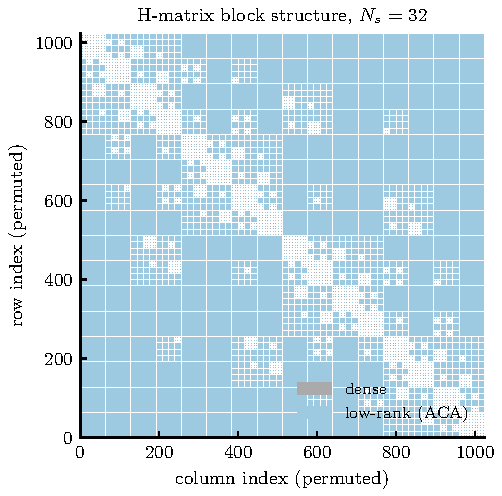
\includegraphics[width=0.94\linewidth]{figures/fig_hmatrix_blocks.pdf}
\end{column}
\end{columns}
\end{frame}

%% ── Slide 4: H-matrix matvec ────────────────────────────────────────────────
\begin{frame}{H-Matrix Matrix–Vector Product}
\begin{columns}[T]
\begin{column}{0.50\textwidth}
  \textbf{Block loop} (OpenMP parallel):
  \vspace{0.3em}

  \begin{tikzpicture}[node distance=4pt]
    % blocks
    \node[block d, minimum width=2.0cm, minimum height=0.55cm,
          draw=mgray, rounded corners=1pt] (d1) {\footnotesize dense $\;D x$};
    \node[block lr, minimum width=2.0cm, minimum height=0.55cm,
          below=of d1, draw=mblue!80, rounded corners=1pt]
         (lr1) {\footnotesize\color{white}low-rank $\;U(Vx)$};
    \node[block d, minimum width=2.0cm, minimum height=0.55cm,
          below=of lr1, draw=mgray, rounded corners=1pt]
         (d2) {\footnotesize dense $\;D x$};
    \node[block lr, minimum width=2.0cm, minimum height=0.55cm,
          below=of d2, draw=mblue!80, rounded corners=1pt]
         (lr2) {\footnotesize\color{white}low-rank $\;U(Vx)$};
    % p vector
    \node[draw=mblue, minimum width=0.5cm, minimum height=2.8cm,
          right=1.2cm of lr1, fill=mlblue!30] (pv)
         {\rotatebox{90}{\footnotesize $p$}};
    % u vector
    \node[draw=mred, minimum width=0.5cm, minimum height=2.8cm,
          left=1.1cm of lr1, fill=mred!15] (uv)
         {\rotatebox{90}{\footnotesize $u\;\mathrel{+}=$}};
    % arrows
    \foreach \blk in {d1,lr1,d2,lr2}{
      \draw[arr,mblue!60] (pv.west) -- (\blk.east);
      \draw[arr,mred!70]  (\blk.west) -- (uv.east);
    }
  \end{tikzpicture}
\end{column}
\begin{column}{0.46\textwidth}
  \[
    u(I) \mathrel{+}= D\,p(J) \quad\text{(dense)}
  \]
  \[
    u(I) \mathrel{+}= U\bigl(V\,p(J)\bigr) \quad\text{(low-rank)}
  \]
  \vspace{0.5em}
  \begin{itemize}
    \item Permute $p$ once before the loop
    \item Each block is \textbf{independent} $\to$ OpenMP
    \item Complexity: $O(N\log^2 N)$
  \end{itemize}
  \vspace{0.4em}
  \textbf{Measured}: $N\!=\!4096$ ($N_s\!=\!64$)\\
  \hspace{1em} assembly: 7\,ms \;|\; matvec: 0.6\,ms
\end{column}
\end{columns}
\end{frame}

%% ── Slide 5: Boussinesq kernel (Love formula) ────────────────────────────────
\begin{frame}{Boussinesq Green's Function: Love Element Formula}
\begin{columns}[T]
\begin{column}{0.54\textwidth}
  Green's function for elastic half-space ($\Esta = E/(1-\nu^2)$):
  \[
    G(\mathbf{r}) = \frac{1}{\pi\Esta |\mathbf{r}|}
  \]
  Discretise on $N_s\!\times\!N_s$ grid of elements of side $h$:
  \[
    S_{ij} = \frac{1}{\pi\Esta}\,\calL\!\left(\Delta x,\Delta y,\tfrac{h}{2}\right)
  \]
  \textbf{Love (1929)} exact integral over a square element:
  {\small
  \begin{align*}
    \calL(x,y,a) &= (x{+}a)\ln\frac{(y{+}a)+R_{++}}{(y{-}a)+R_{+-}}
                 +(y{+}a)\ln\frac{(x{+}a)+R_{++}}{(x{-}a)+R_{-+}} \\
                 &\quad+(x{-}a)\ln\frac{(y{-}a)+R_{--}}{(y{+}a)+R_{-+}}
                 +(y{-}a)\ln\frac{(x{-}a)+R_{--}}{(x{+}a)+R_{+-}}
  \end{align*}
  }
  \alert{Self-term}: $S_{ii} = \dfrac{4h\ln(1{+}\sqrt{2})}{\pi\Esta}$
\end{column}
\begin{column}{0.42\textwidth}
  \centering
  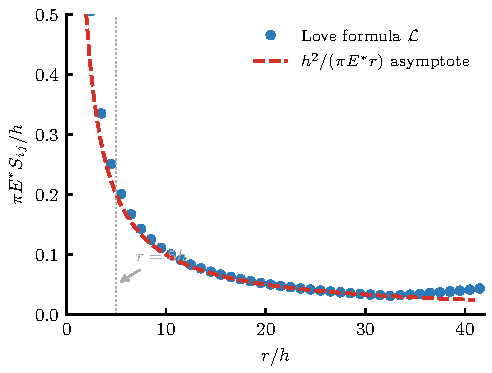
\includegraphics[width=\linewidth]{figures/fig_kernel_decay.pdf}
  \vspace{0.3em}
  {\small 3.7\,\% deviation at $r=h$; below 0.2\,\% at $r\ge5h$}
\end{column}
\end{columns}
\end{frame}
